\section{Experiments}
\label{sec:experiments}

We evaluate MASOpt on eight benchmarks and study the roles of diagnostic and verification experience, prompt quality, workflow architecture, and backbone model. The comparisons distinguish published baselines, selected system configurations, and exploratory follow-up analyses; detailed protocols are collected in Appendix~\ref{app:experimental-details}.

\subsection{Experimental Setup}
\label{sec:experimental-setup}

\paragraph{Benchmarks.}
We evaluate MASOpt on eight benchmarks spanning four domains: code generation (HumanEval and MBPP), mathematical reasoning (GSM8K and MATH Level-5), reading comprehension (HotpotQA and DROP), and interactive task completion (ALFWorld and TextCraft) \citep{chen2021humaneval,austin2021mbpp,cobbe2021gsm8k,hendrycks2021math,yang2018hotpotqa,dua2019drop,shridhar2020alfworld,prasad2024textcraft}. This suite tests both final-answer quality and adaptation to evolving environment feedback. Dataset sizes, splits, and the MATH subset composition are provided in Appendix~\ref{app:data-splits}.

\paragraph{Baselines.}
We compare three groups of methods: direct and reasoning-based prompting (IO, CoT, and ReAct), prompt optimization (PromptBreeder, Instinct, MIPRO, and MASPOB), and workflow generation or adaptation (AFlow and HiveMind). References are given alongside the methods in Table~\ref{tab:main-results}. The eight IO--MASPOB results are published means reported by \citet{hong2026maspob}; HiveMind is our unofficial three-node transfer from its original financial-trading setting. Within-system analyses compare MASOpt with the same locally executed workflow. Protocol and selection differences are documented in Appendix~\ref{app:protocols}.

\paragraph{Metrics.}
We report pass@1 on HumanEval and MBPP, answer accuracy on GSM8K and MATH, normalized F1 on HotpotQA and DROP, and native task success rate on ALFWorld and TextCraft. Internal generation branches and repair attempts do not count as additional submissions for pass@1. Task scores use a 0--100 scale, and differences are expressed in percentage points (pp); each table average weights its benchmark columns equally. Prompt quality is assessed separately with a 0--10 rubric and anonymous paired evaluation in both presentation orders.

\paragraph{Implementation details.}
Unless otherwise stated, local main, component, and architecture experiments request \texttt{gpt-4o-mini-2024-07-18} with temperature 0 and top-$p$ 1; the provider generally returns the \texttt{gpt-4o-mini} alias, so the served snapshot is not independently verified. Backbone parameters remain fixed, and hidden answers are excluded from online acceptance decisions. ALFWorld and TextCraft use 35- and 20-step limits, respectively, with at most two repair proposals in the controlled TextCraft runs. Local scores normally summarize one complete prediction set, and the main MASOpt row selects the highest completed score per task. Because some development used test-set feedback, these results characterize the recorded systems rather than an untouched holdout; split allocations, model-selection history, and budget differences are detailed in Appendix~\ref{app:protocols}.

\subsection{Main Results}
\label{sec:main-results}

\begin{table}[!htbp]
    \centering
    \setlength{\belowcaptionskip}{6pt}
    \caption{Performance (\%) on six non-interactive benchmarks. Baselines are ordered by increasing reported average; MASOpt is separated and bolded. All baselines except HiveMind use published means from \citet{hong2026maspob}, with dispersion omitted; HiveMind is a local adaptation. MASOpt reports selected completed configurations. Avg. is the unweighted six-benchmark mean. See Appendix~\ref{app:protocols} for comparability limits.}
    \label{tab:main-results}
    \scriptsize
    \setlength{\tabcolsep}{3.7pt}
    \resizebox{\textwidth}{!}{%
    \begin{tabular}{@{}lccccccc@{}}
        \toprule
        Method & HumanEval & MBPP & GSM8K & MATH & HotpotQA & DROP & Avg. \\
        \midrule
        IO (GPT-4o-mini) & 89.31 & 69.11 & 87.80 & 51.71 & 60.36 & 53.09 & 68.56 \\
        CoT \citep{wei2022cot} & 89.57 & 69.89 & 88.34 & 52.47 & 67.62 & 58.27 & 71.03 \\
        ReAct \citep{yao2023react} & 87.79 & 66.08 & 88.91 & 52.61 & 65.61 & 67.25 & 71.38 \\
        PromptBreeder \citep{fernando2024promptbreeder} & 88.80 & 70.38 & 91.97 & 52.13 & 68.76 & 71.85 & 73.98 \\
        Instinct \citep{lin2023instinct} & 90.08 & 70.23 & 92.64 & 52.40 & 69.92 & 71.90 & 74.53 \\
        AFlow \citep{zhang2024aflow} & 91.09 & 79.96 & 93.36 & 53.83 & 73.42 & 79.48 & 78.52 \\
        MIPRO \citep{opsahlong2024mipro} & 91.35 & 80.65 & 92.80 & 54.90 & 74.37 & 79.13 & 78.87 \\
        HiveMind \citep{xia2025hivemind} & 89.31 & 71.55 & 92.99 & 57.41 & 67.23 & 68.76 & 74.54 \\
        MASPOB \citep{hong2026maspob} & 94.15 & 80.65 & 93.90 & 57.05 & 75.43 & 82.28 & 80.58 \\
        \midrule
        \textbf{MASOpt} & \textbf{96.95} & \textbf{84.16} & \textbf{94.41} & \textbf{62.76} & \textbf{76.49} & \textbf{85.66} & \textbf{83.40} \\
        \bottomrule
    \end{tabular}}
\end{table}

\paragraph{Observation 1: Broad performance gains across non-interactive tasks.}
Table~\ref{tab:main-results} shows that the selected MASOpt configurations attain the highest reported score on all six benchmarks, with an average of 83.40 versus 80.58 for MASPOB. Relative to MASPOB, the gains are 2.80/3.51 pp on HumanEval/MBPP, 0.51/5.71 pp on GSM8K/MATH, and 1.06/3.38 pp on HotpotQA/DROP. The larger gains on MATH and MBPP contrast with the smaller margin on GSM8K, where the baseline already reaches 93.90. This pattern is consistent with task-dependent opportunities for local repair. These are descriptive comparisons of selected MASOpt configurations with published baseline means, not a matched statistical test.

\begin{wraptable}{r}{0.50\textwidth}
    \vspace{-\intextsep}
    \centering
    \caption{Interactive success rate (\%). Avg. weights the three score columns equally. ALFWorld uses historical archives; TextCraft uses the shared action interface. Protocol differences are detailed in Appendix~\ref{app:interactive-protocols}.}
    \label{tab:interactive-results}
    \small
    \setlength{\tabcolsep}{2.3pt}
    \renewcommand{\arraystretch}{1.04}
    \begin{tabular*}{\linewidth}{@{\extracolsep{\fill}}lrrrr@{}}
        \toprule
        & \multicolumn{2}{c}{ALFWorld} & & \\
        \cmidrule(lr){2-3}
        Method & Seen & Unseen & TextCraft & Avg. \\
        \midrule
        HiveMind & 28.57 & 27.61 & 12.50 & 22.89 \\
        MASPOB & 47.86 & 50.75 & 13.75 & 37.45 \\
        MIPRO & 51.43 & 50.00 & 12.50 & 37.98 \\
        AFlow & 50.71 & 54.48 & 12.50 & 39.23 \\
        \midrule
        \textbf{MASOpt} & \textbf{75.00} & \textbf{89.55} & \textbf{30.00} & \textbf{64.85} \\
        \bottomrule
    \end{tabular*}
    \vspace{-0.5\baselineskip}
\end{wraptable}

\paragraph{Observation 2: Higher recorded success on interactive tasks.}
Table~\ref{tab:interactive-results} extends the comparison to sequential decisions. MASOpt solves 24 of 80 TextCraft tasks (30.00\%), compared with 10 for MIPRO and 11 for the simplified MASPOB adaptation, under the shared typed action interface and 20-step limit. Its historical ALFWorld scores are 75.00\% on seen tasks and 89.55\% on unseen tasks, giving a three-column average of 64.85. These observations motivate local repair from dependency, inventory, and environment feedback. However, the ALFWorld baseline names identify seed-plus-memory archives with identical role prompts, not distinct optimizer executions; a later MASOpt rerun reaches 84.33\% on unseen tasks. Appendix~\ref{app:interactive-protocols} reports these distinctions and the associated interaction costs, so the historical margins should not be read as controlled algorithmic gains.

\FloatBarrier
\subsection{Contribution of Diagnostic and Verification Experience}
\label{sec:experience-ablation}

We examine whether learned experience helps the controller locate failures and decide which repairs to retain. This study separates the contribution of diagnostic and verification experience from the effect of simply invoking the three-agent control loop.

\begin{figure}[!htbp]
    \centering
    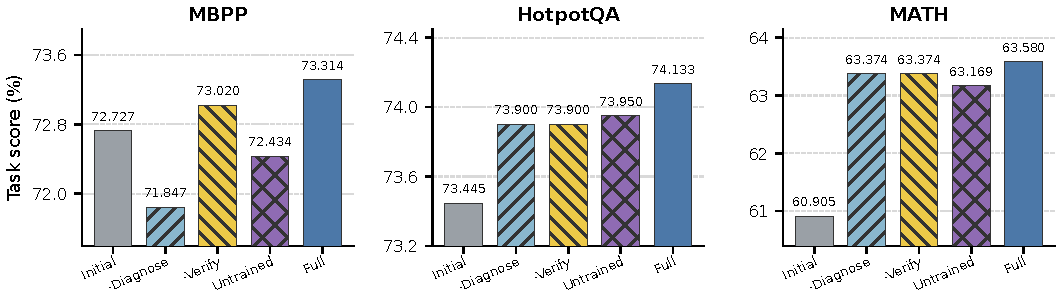
\includegraphics[width=0.94\textwidth]{figures/ablation_experience.pdf}
    \caption{Experience ablations on MBPP (341 tasks), HotpotQA (800), and MATH (486). Each panel uses a dataset-specific truncated vertical axis to make sub-point differences visible; bar labels are rounded to three decimals. GSM8K is omitted because its separately registered controller is not structurally identical to these three runs.}
    \label{fig:experience-ablation}
\end{figure}

We compare Full with variants that remove diagnostic experience, verification experience, or all learned experience while retaining the controller and its underlying workflow. All variants share the same configuration-specific Initial outputs. As shown in Figure~\ref{fig:experience-ablation}, Full improves over Initial by 0.59, 0.69, and 2.67 pp on MBPP, HotpotQA, and MATH, and exceeds the strongest displayed ablation by 0.29, 0.18, and 0.21 pp. Removing diagnostic experience produces the largest MBPP decrease (1.47 pp); on MATH, removing either diagnostic or verification experience changes only one correct answer. Thus, the recorded benefit varies by task and is modest in several comparisons. These post-hoc results are exploratory; configuration-specific baselines, fallback behavior, and the separate GSM8K analysis are documented in Appendix~\ref{app:experience-details}.

\begin{figure}[!htbp]
    \centering
    \begin{minipage}[t]{0.49\textwidth}
        \vspace{0pt}
        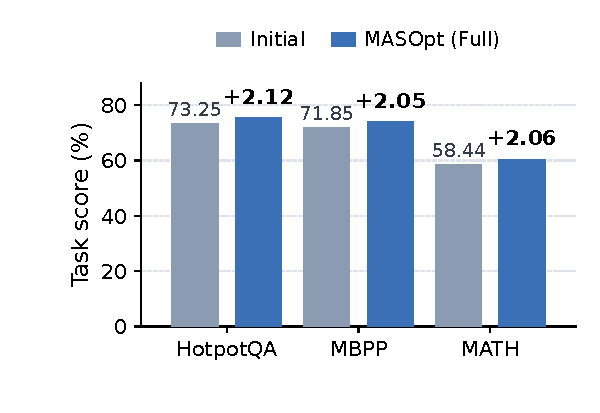
\includegraphics[width=\linewidth]{figures/architecture_adaptation.pdf}
        \caption{Adaptation to three alternative workflows. Gray bars show Initial and blue bars Full; labels give Initial scores and Full-minus-Initial gains in pp.}
        \label{fig:architecture-adaptation}
    \end{minipage}\hfill
    \begin{minipage}[t]{0.49\textwidth}
        \vspace{0pt}
        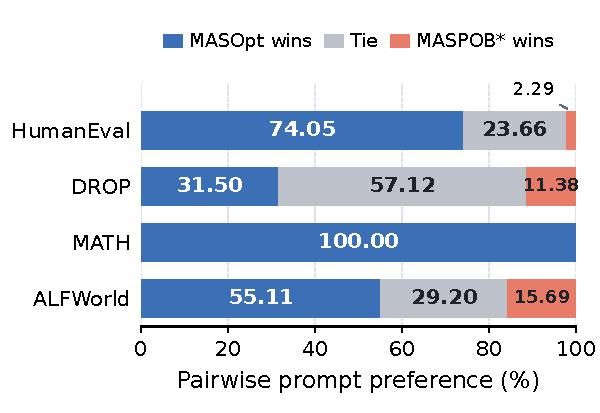
\includegraphics[width=\linewidth]{figures/prompt_quality.pdf}
        \caption{Pairwise prompt preference on four datasets. Segments show MASOpt wins, ties, and MASPOB* wins; zero-width segments are omitted.}
        \label{fig:prompt-quality}
    \end{minipage}
\end{figure}

\subsection{Pairwise Prompt Quality}
\label{sec:prompt-quality}

We examine whether MASOpt prompts are preferred under a fixed rubric independently of final task success. This study compares paired prompts on HumanEval, DROP, MATH, and ALFWorld to assess instruction quality across code generation, reading comprehension, mathematical reasoning, and interactive decision-making.

A GPT-5.6-sol judge scores anonymized prompts in both A/B and B/A orders on six 0--10 dimensions. We average the two overall-quality scores for each prompt; a MASOpt-minus-baseline difference above 0.5 is a win, below $-0.5$ is a loss, and otherwise is a tie. MASPOB* uses the published optimized prompts on the three non-interactive datasets and a seed-plus-memory archive on ALFWorld. Figure~\ref{fig:prompt-quality} shows MASOpt win rates of 74.05\%, 31.50\%, 100.00\%, and 55.11\%, respectively. MATH receives uniform preference, while DROP is dominated by ties (57.12\%), indicating a weaker separation under the rubric. On ALFWorld, MASOpt wins exceed baseline wins (15.69\%), with 29.20\% ties. These selected-dataset comparisons provide evidence about judged prompt quality, not task success; a single evaluator and presentation-order sensitivity limit the strength of the conclusion.

\subsection{Adaptation to Alternative Workflow Architectures}
\label{sec:architecture-adaptation}

We test whether MASOpt remains useful when the underlying workflow is simplified. By holding the backbone and task set fixed while changing the branch structure, this study examines the controller's applicability beyond the original workflow configuration.

We use one \textsc{AnswerGenerate} call followed by \textsc{FormatAnswer} on HotpotQA, one \textsc{CodeGenerate} branch followed by test and repair on MBPP, and two text solvers with \textsc{ScEnsemble} but no program branch on MATH. Initial executes each alternative workflow directly; Full applies MASOpt to the same workflow. Figure~\ref{fig:architecture-adaptation} compares the fixed Initial scores with the latest Full results: 73.2481 to 75.3711 on HotpotQA, 71.8475 to 73.9003 on MBPP, and 58.4362 to 60.4938 on MATH. The corresponding gains are 2.12, 2.05, and 2.06 pp. The similar positive margins suggest that local repair remains useful across these three branch structures. The recorded configurations include post-hoc policy choices and execution recovery, so the comparison supports applicability to the tested workflows rather than architecture-independent improvement under a uniform budget.

\FloatBarrier
\subsection{Adaptation Across Backbone Models}
\label{sec:backbone-adaptation}

We examine whether MASOpt can be instantiated with different backbone models while retaining the same online repair mechanism. This study characterizes model-specific adaptation across six benchmarks, rather than assuming that a controller calibrated for one backbone transfers unchanged.

\begin{figure}[!htbp]
    \centering
    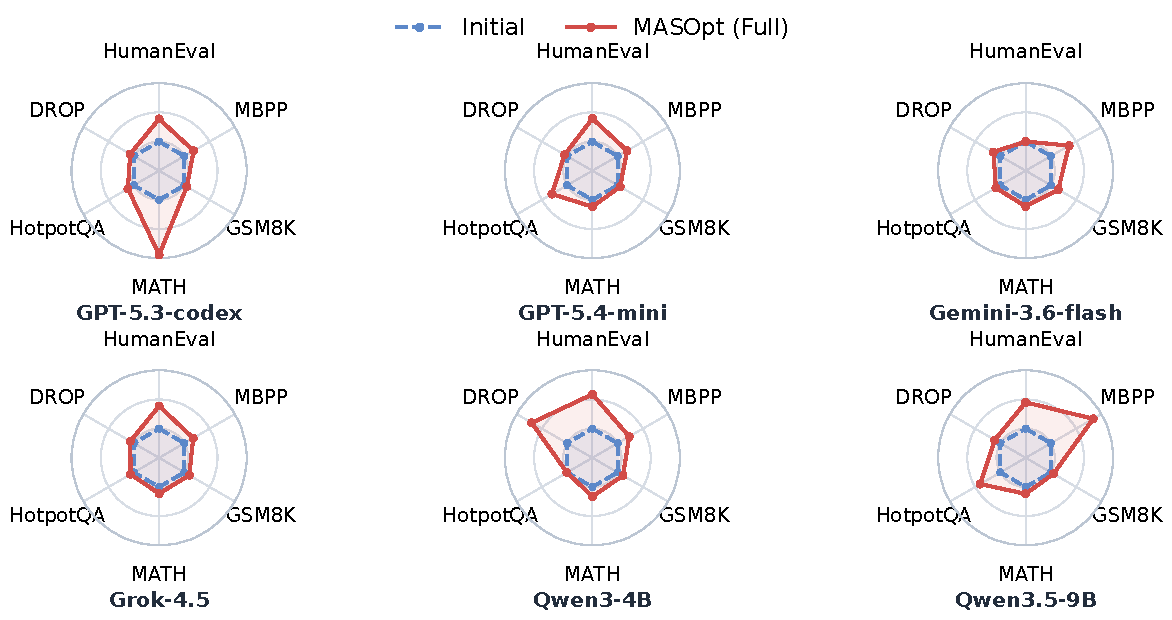
\includegraphics[width=\textwidth]{figures/backbone_radar.pdf}
    \caption{Adaptation across six backbones. Each Initial score is normalized to 100; all panels use the same 99--102 radial range to resolve small differences.}
    \label{fig:backbone-radar}
\end{figure}

We pair each model-specific Initial workflow with its Full counterpart on HumanEval, MBPP, GSM8K, MATH, HotpotQA, and DROP. Figure~\ref{fig:backbone-radar} compares the six backbones under these paired configurations. Full improves in 35 of 36 model--task pairs and ties Gemini-3.6-flash on HumanEval, where Initial already reaches 100\%. Mean gains across the six tasks range from 0.25 to 0.51 pp across backbones. The pattern shows broadly positive but modest and task-dependent changes. Experience, recovery policies, and execution budgets differ across configurations, so these results support model-specific applicability rather than controlled transfer or statistically significant improvement under a common protocol. Appendix~\ref{app:backbone-protocols} details these differences.

\FloatBarrier
